% Options for packages loaded elsewhere
% Options for packages loaded elsewhere
\PassOptionsToPackage{unicode}{hyperref}
\PassOptionsToPackage{hyphens}{url}
%
\documentclass[
  spanish,
  letterpaper,
]{book}
\usepackage{xcolor}
\usepackage[margin=1in]{geometry}
\usepackage{amsmath,amssymb}
\setcounter{secnumdepth}{5}
\usepackage{iftex}
\ifPDFTeX
  \usepackage[T1]{fontenc}
  \usepackage[utf8]{inputenc}
  \usepackage{textcomp} % provide euro and other symbols
\else % if luatex or xetex
  \usepackage{unicode-math} % this also loads fontspec
  \defaultfontfeatures{Scale=MatchLowercase}
  \defaultfontfeatures[\rmfamily]{Ligatures=TeX,Scale=1}
\fi
\usepackage{lmodern}
\ifPDFTeX\else
  % xetex/luatex font selection
\fi
% Use upquote if available, for straight quotes in verbatim environments
\IfFileExists{upquote.sty}{\usepackage{upquote}}{}
\IfFileExists{microtype.sty}{% use microtype if available
  \usepackage[]{microtype}
  \UseMicrotypeSet[protrusion]{basicmath} % disable protrusion for tt fonts
}{}
\makeatletter
\@ifundefined{KOMAClassName}{% if non-KOMA class
  \IfFileExists{parskip.sty}{%
    \usepackage{parskip}
  }{% else
    \setlength{\parindent}{0pt}
    \setlength{\parskip}{6pt plus 2pt minus 1pt}}
}{% if KOMA class
  \KOMAoptions{parskip=half}}
\makeatother
% Make \paragraph and \subparagraph free-standing
\makeatletter
\ifx\paragraph\undefined\else
  \let\oldparagraph\paragraph
  \renewcommand{\paragraph}{
    \@ifstar
      \xxxParagraphStar
      \xxxParagraphNoStar
  }
  \newcommand{\xxxParagraphStar}[1]{\oldparagraph*{#1}\mbox{}}
  \newcommand{\xxxParagraphNoStar}[1]{\oldparagraph{#1}\mbox{}}
\fi
\ifx\subparagraph\undefined\else
  \let\oldsubparagraph\subparagraph
  \renewcommand{\subparagraph}{
    \@ifstar
      \xxxSubParagraphStar
      \xxxSubParagraphNoStar
  }
  \newcommand{\xxxSubParagraphStar}[1]{\oldsubparagraph*{#1}\mbox{}}
  \newcommand{\xxxSubParagraphNoStar}[1]{\oldsubparagraph{#1}\mbox{}}
\fi
\makeatother

\usepackage{color}
\usepackage{fancyvrb}
\newcommand{\VerbBar}{|}
\newcommand{\VERB}{\Verb[commandchars=\\\{\}]}
\DefineVerbatimEnvironment{Highlighting}{Verbatim}{commandchars=\\\{\}}
% Add ',fontsize=\small' for more characters per line
\usepackage{framed}
\definecolor{shadecolor}{RGB}{241,243,245}
\newenvironment{Shaded}{\begin{snugshade}}{\end{snugshade}}
\newcommand{\AlertTok}[1]{\textcolor[rgb]{0.68,0.00,0.00}{#1}}
\newcommand{\AnnotationTok}[1]{\textcolor[rgb]{0.37,0.37,0.37}{#1}}
\newcommand{\AttributeTok}[1]{\textcolor[rgb]{0.40,0.45,0.13}{#1}}
\newcommand{\BaseNTok}[1]{\textcolor[rgb]{0.68,0.00,0.00}{#1}}
\newcommand{\BuiltInTok}[1]{\textcolor[rgb]{0.00,0.23,0.31}{#1}}
\newcommand{\CharTok}[1]{\textcolor[rgb]{0.13,0.47,0.30}{#1}}
\newcommand{\CommentTok}[1]{\textcolor[rgb]{0.37,0.37,0.37}{#1}}
\newcommand{\CommentVarTok}[1]{\textcolor[rgb]{0.37,0.37,0.37}{\textit{#1}}}
\newcommand{\ConstantTok}[1]{\textcolor[rgb]{0.56,0.35,0.01}{#1}}
\newcommand{\ControlFlowTok}[1]{\textcolor[rgb]{0.00,0.23,0.31}{\textbf{#1}}}
\newcommand{\DataTypeTok}[1]{\textcolor[rgb]{0.68,0.00,0.00}{#1}}
\newcommand{\DecValTok}[1]{\textcolor[rgb]{0.68,0.00,0.00}{#1}}
\newcommand{\DocumentationTok}[1]{\textcolor[rgb]{0.37,0.37,0.37}{\textit{#1}}}
\newcommand{\ErrorTok}[1]{\textcolor[rgb]{0.68,0.00,0.00}{#1}}
\newcommand{\ExtensionTok}[1]{\textcolor[rgb]{0.00,0.23,0.31}{#1}}
\newcommand{\FloatTok}[1]{\textcolor[rgb]{0.68,0.00,0.00}{#1}}
\newcommand{\FunctionTok}[1]{\textcolor[rgb]{0.28,0.35,0.67}{#1}}
\newcommand{\ImportTok}[1]{\textcolor[rgb]{0.00,0.46,0.62}{#1}}
\newcommand{\InformationTok}[1]{\textcolor[rgb]{0.37,0.37,0.37}{#1}}
\newcommand{\KeywordTok}[1]{\textcolor[rgb]{0.00,0.23,0.31}{\textbf{#1}}}
\newcommand{\NormalTok}[1]{\textcolor[rgb]{0.00,0.23,0.31}{#1}}
\newcommand{\OperatorTok}[1]{\textcolor[rgb]{0.37,0.37,0.37}{#1}}
\newcommand{\OtherTok}[1]{\textcolor[rgb]{0.00,0.23,0.31}{#1}}
\newcommand{\PreprocessorTok}[1]{\textcolor[rgb]{0.68,0.00,0.00}{#1}}
\newcommand{\RegionMarkerTok}[1]{\textcolor[rgb]{0.00,0.23,0.31}{#1}}
\newcommand{\SpecialCharTok}[1]{\textcolor[rgb]{0.37,0.37,0.37}{#1}}
\newcommand{\SpecialStringTok}[1]{\textcolor[rgb]{0.13,0.47,0.30}{#1}}
\newcommand{\StringTok}[1]{\textcolor[rgb]{0.13,0.47,0.30}{#1}}
\newcommand{\VariableTok}[1]{\textcolor[rgb]{0.07,0.07,0.07}{#1}}
\newcommand{\VerbatimStringTok}[1]{\textcolor[rgb]{0.13,0.47,0.30}{#1}}
\newcommand{\WarningTok}[1]{\textcolor[rgb]{0.37,0.37,0.37}{\textit{#1}}}

\usepackage{longtable,booktabs,array}
\usepackage{calc} % for calculating minipage widths
% Correct order of tables after \paragraph or \subparagraph
\usepackage{etoolbox}
\makeatletter
\patchcmd\longtable{\par}{\if@noskipsec\mbox{}\fi\par}{}{}
\makeatother
% Allow footnotes in longtable head/foot
\IfFileExists{footnotehyper.sty}{\usepackage{footnotehyper}}{\usepackage{footnote}}
\makesavenoteenv{longtable}
\usepackage{graphicx}
\makeatletter
\newsavebox\pandoc@box
\newcommand*\pandocbounded[1]{% scales image to fit in text height/width
  \sbox\pandoc@box{#1}%
  \Gscale@div\@tempa{\textheight}{\dimexpr\ht\pandoc@box+\dp\pandoc@box\relax}%
  \Gscale@div\@tempb{\linewidth}{\wd\pandoc@box}%
  \ifdim\@tempb\p@<\@tempa\p@\let\@tempa\@tempb\fi% select the smaller of both
  \ifdim\@tempa\p@<\p@\scalebox{\@tempa}{\usebox\pandoc@box}%
  \else\usebox{\pandoc@box}%
  \fi%
}
% Set default figure placement to htbp
\def\fps@figure{htbp}
\makeatother


% definitions for citeproc citations
\NewDocumentCommand\citeproctext{}{}
\NewDocumentCommand\citeproc{mm}{%
  \begingroup\def\citeproctext{#2}\cite{#1}\endgroup}
\makeatletter
 % allow citations to break across lines
 \let\@cite@ofmt\@firstofone
 % avoid brackets around text for \cite:
 \def\@biblabel#1{}
 \def\@cite#1#2{{#1\if@tempswa , #2\fi}}
\makeatother
\newlength{\cslhangindent}
\setlength{\cslhangindent}{1.5em}
\newlength{\csllabelwidth}
\setlength{\csllabelwidth}{3em}
\newenvironment{CSLReferences}[2] % #1 hanging-indent, #2 entry-spacing
 {\begin{list}{}{%
  \setlength{\itemindent}{0pt}
  \setlength{\leftmargin}{0pt}
  \setlength{\parsep}{0pt}
  % turn on hanging indent if param 1 is 1
  \ifodd #1
   \setlength{\leftmargin}{\cslhangindent}
   \setlength{\itemindent}{-1\cslhangindent}
  \fi
  % set entry spacing
  \setlength{\itemsep}{#2\baselineskip}}}
 {\end{list}}
\usepackage{calc}
\newcommand{\CSLBlock}[1]{\hfill\break\parbox[t]{\linewidth}{\strut\ignorespaces#1\strut}}
\newcommand{\CSLLeftMargin}[1]{\parbox[t]{\csllabelwidth}{\strut#1\strut}}
\newcommand{\CSLRightInline}[1]{\parbox[t]{\linewidth - \csllabelwidth}{\strut#1\strut}}
\newcommand{\CSLIndent}[1]{\hspace{\cslhangindent}#1}

\ifLuaTeX
\usepackage[bidi=basic]{babel}
\else
\usepackage[bidi=default]{babel}
\fi
% get rid of language-specific shorthands (see #6817):
\let\LanguageShortHands\languageshorthands
\def\languageshorthands#1{}


\setlength{\emergencystretch}{3em} % prevent overfull lines

\providecommand{\tightlist}{%
  \setlength{\itemsep}{0pt}\setlength{\parskip}{0pt}}



 


\makeatletter
\@ifpackageloaded{tcolorbox}{}{\usepackage[skins,breakable]{tcolorbox}}
\@ifpackageloaded{fontawesome5}{}{\usepackage{fontawesome5}}
\definecolor{quarto-callout-color}{HTML}{909090}
\definecolor{quarto-callout-note-color}{HTML}{0758E5}
\definecolor{quarto-callout-important-color}{HTML}{CC1914}
\definecolor{quarto-callout-warning-color}{HTML}{EB9113}
\definecolor{quarto-callout-tip-color}{HTML}{00A047}
\definecolor{quarto-callout-caution-color}{HTML}{FC5300}
\definecolor{quarto-callout-color-frame}{HTML}{acacac}
\definecolor{quarto-callout-note-color-frame}{HTML}{4582ec}
\definecolor{quarto-callout-important-color-frame}{HTML}{d9534f}
\definecolor{quarto-callout-warning-color-frame}{HTML}{f0ad4e}
\definecolor{quarto-callout-tip-color-frame}{HTML}{02b875}
\definecolor{quarto-callout-caution-color-frame}{HTML}{fd7e14}
\makeatother
\makeatletter
\@ifpackageloaded{bookmark}{}{\usepackage{bookmark}}
\makeatother
\makeatletter
\@ifpackageloaded{caption}{}{\usepackage{caption}}
\AtBeginDocument{%
\ifdefined\contentsname
  \renewcommand*\contentsname{Tabla de contenidos}
\else
  \newcommand\contentsname{Tabla de contenidos}
\fi
\ifdefined\listfigurename
  \renewcommand*\listfigurename{Listado de Figuras}
\else
  \newcommand\listfigurename{Listado de Figuras}
\fi
\ifdefined\listtablename
  \renewcommand*\listtablename{Listado de Tablas}
\else
  \newcommand\listtablename{Listado de Tablas}
\fi
\ifdefined\figurename
  \renewcommand*\figurename{Figura}
\else
  \newcommand\figurename{Figura}
\fi
\ifdefined\tablename
  \renewcommand*\tablename{Tabla}
\else
  \newcommand\tablename{Tabla}
\fi
}
\@ifpackageloaded{float}{}{\usepackage{float}}
\floatstyle{ruled}
\@ifundefined{c@chapter}{\newfloat{codelisting}{h}{lop}}{\newfloat{codelisting}{h}{lop}[chapter]}
\floatname{codelisting}{Listado}
\newcommand*\listoflistings{\listof{codelisting}{Listado de Listados}}
\makeatother
\makeatletter
\makeatother
\makeatletter
\@ifpackageloaded{caption}{}{\usepackage{caption}}
\@ifpackageloaded{subcaption}{}{\usepackage{subcaption}}
\makeatother
\usepackage{bookmark}
\IfFileExists{xurl.sty}{\usepackage{xurl}}{} % add URL line breaks if available
\urlstyle{same}
\hypersetup{
  pdftitle={Libro de Investigaciones},
  pdfauthor={Mauricio Romero},
  pdflang={es},
  hidelinks,
  pdfcreator={LaTeX via pandoc}}


\title{Libro de Investigaciones}
\usepackage{etoolbox}
\makeatletter
\providecommand{\subtitle}[1]{% add subtitle to \maketitle
  \apptocmd{\@title}{\par {\large #1 \par}}{}{}
}
\makeatother
\subtitle{Una colección de artículos científicos y estudios de
investigación}
\author{Mauricio Romero}
\date{2025-09-01}
\begin{document}
\frontmatter
\maketitle

\renewcommand*\contentsname{Tabla de contenidos}
{
\setcounter{tocdepth}{2}
\tableofcontents
}

\mainmatter
\bookmarksetup{startatroot}

\chapter*{Inicio}\label{inicio}
\addcontentsline{toc}{chapter}{Inicio}

\markboth{Inicio}{Inicio}

Bienvenido al \textbf{Libro de Investigaciones}, una colección de
capítulos de investigación organizados en capítulos independientes.

\bookmarksetup{startatroot}

\chapter*{Contenido}\label{contenido}
\addcontentsline{toc}{chapter}{Contenido}

\markboth{Contenido}{Contenido}

\section*{Capítulo 1: La Palma Seismicity
2021}\label{capuxedtulo-1-la-palma-seismicity-2021}
\addcontentsline{toc}{section}{Capítulo 1: La Palma Seismicity 2021}

\markright{Capítulo 1: La Palma Seismicity 2021}

En septiembre de 2021, un salto significativo en la actividad sísmica en
la isla de La Palma (Islas Canarias, España) señaló el comienzo de una
crisis volcánica. Este estudio analiza los datos de terremotos
recopilados y publicados por el Instituto Geográfico Nacional (IGN),
revelando sismicidad que se origina en dos profundidades distintas.

\section*{Capítulo 2: Evaluating the Transfer of Information in Phase
Retrieval STEM
Techniques}\label{capuxedtulo-2-evaluating-the-transfer-of-information-in-phase-retrieval-stem-techniques}
\addcontentsline{toc}{section}{Capítulo 2: Evaluating the Transfer of
Information in Phase Retrieval STEM Techniques}

\markright{Capítulo 2: Evaluating the Transfer of Information in Phase
Retrieval STEM Techniques}

Este estudio evalúa métodos de recuperación de fase en microscopía
electrónica de transmisión de barrido (STEM), analizando técnicas como
imágenes del centro de masa, STEM de campo brillante corregido por
inclinación y métodos ptychográficos directos.

\section*{Arquitectura del Proyecto}\label{arquitectura-del-proyecto}
\addcontentsline{toc}{section}{Arquitectura del Proyecto}

\markright{Arquitectura del Proyecto}

Esta implementación en \textbf{Quarto} ofrece:

\begin{itemize}
\tightlist
\item
  ✅ \textbf{Estabilidad garantizada}: Servidor web confiable y
  funcional
\item
  ✅ \textbf{Navegación fluida}: Enlaces internos que funcionan
  correctamente
\item
  ✅ \textbf{Formato científico}: Soporte nativo para ecuaciones,
  referencias y figuras
\item
  ✅ \textbf{Exports múltiples}: HTML interactivo y PDF profesional
\item
  ✅ \textbf{Live preview}: Actualización automática durante edición
\item
  ✅ \textbf{Mantenimiento sencillo}: Configuración simple y robusta
\end{itemize}

\section*{Navegación}\label{navegaciuxf3n}
\addcontentsline{toc}{section}{Navegación}

\markright{Navegación}

Utiliza la navegación lateral o los enlaces de capítulos para explorar
los diferentes estudios de investigación incluidos en este libro.

\bookmarksetup{startatroot}

\chapter{1. Terremotos de La Palma: Análisis sísmico de la actividad
volcánica}\label{terremotos-de-la-palma-anuxe1lisis-suxedsmico-de-la-actividad-volcuxe1nica}

\phantomsection\label{resumen}
\bookmarksetup{startatroot}

\chapter{Resumen}\label{resumen}

Este estudio analiza la actividad sísmica asociada a la erupción
volcánica de La Palma de 2021 para investigar la existencia de sistemas
magmáticos multireservorio. Utilizando datos sísmicos del Instituto
Geográfico Nacional, examinamos patrones espaciales y temporales de
sismicidad para validar modelos teóricos de almacenamiento y transporte
de magma. Nuestro análisis de 5465 eventos sísmicos revela una
agrupación distintiva a profundidades superficiales (10-15 km) y
profundas (30-40 km), lo que proporciona evidencia sólida de la
existencia de reservorios magmáticos tanto en la corteza como en el
manto que alimentan el sistema volcánico de Cumbre Vieja

\phantomsection\label{abstract}
\bookmarksetup{startatroot}

\chapter{La Palma Earthquakes: Seismic Analysis of Volcanic
Activity}\label{la-palma-earthquakes-seismic-analysis-of-volcanic-activity}

\textbf{Abstract}. This study analyzes seismic activity associated with
the 2021 La Palma volcanic eruption to investigate evidence for proposed
multi-reservoir magma systems. Using earthquake data from the Instituto
Geográfico Nacional, we examine spatial and temporal patterns of
seismicity to validate theoretical models of magma storage and
transport. Our analysis of 5,465 seismic events reveals distinct
clustering at shallow (10-15 km) and deep (30-40 km) depths, providing
strong evidence for both crustal and mantle magma reservoirs feeding the
Cumbre Vieja volcanic system.

\bookmarksetup{startatroot}

\chapter{1. INTRODUCCIÓN}\label{introducciuxf3n}

La Palma, situated in the westernmost region of the Canary Islands
archipelago, represents one of Earth's most active volcanic systems.
Located approximately 100 km from the African coast, this Spanish
territory exemplifies ongoing oceanic island formation processes. The
island's geological evolution has been dominated by multiple phases of
volcanism, with the \emph{Cumbre Vieja} volcanic ridge---a north-south
oriented structure comprising the southern half of the
island---representing the most recent and currently active phase
{[}1,2{]}.

Understanding volcanic earthquake patterns is crucial for eruption
forecasting and hazard assessment. The 2021 eruption of Cumbre Vieja
provided an exceptional opportunity to study real-time seismic
signatures associated with magma movement through proposed
multi-reservoir systems {[}1{]}.

\section{1.1 Historical Context and Volcanic
Setting}\label{historical-context-and-volcanic-setting}

\subsection{Eruption History}\label{eruption-history}

The historical volcanic record of La Palma spans over five centuries,
providing valuable insights into the long-term behavior of the Cumbre
Vieja system. Since European colonization in the late 1400s, eight major
eruptions have been documented, establishing patterns crucial for
probabilistic hazard assessment.

\begin{longtable}[]{@{}cc@{}}
\caption{Recent historic eruptions on La
Palma.}\label{tbl-Tabla1}\tabularnewline
\toprule\noalign{}
Name & Year \\
\midrule\noalign{}
\endfirsthead
\toprule\noalign{}
Name & Year \\
\midrule\noalign{}
\endhead
\bottomrule\noalign{}
\endlastfoot
Current & 2021 \\
Teneguía & 1971 \\
Nambroque & 1949 \\
El Charco & 1712 \\
Volcán San Antonio & 1677 \\
Volcán San Martin & 1646 \\
Tajuya near El Paso & 1585 \\
Montaña Quemada & 1492 \\
\end{longtable}

This equates to an eruption on average every 79 years up until the 1971
event Tabla~\ref{tbl-Tabla1}. The probability of a future eruption can
be modeled by a Poisson distribution:

\[
p(x)=\frac{e^{-\lambda} \lambda^{x}}{x !}
\]

Where \(\lambda\) is the number of eruptions per year,
\(\lambda=\frac{1}{79}\) in this case. The probability of a future
eruption in the next \(t\) years can be calculated by:

\[
p_e = 1-\mathrm{e}^{-t \lambda}
\]

So following the 1971 eruption the probability of an eruption in the
following 50 years --- the period ending this year --- was 0.469. After
the event, the number of eruptions per year moves to
\(\lambda=\frac{1}{75}\) and the probability of a further eruption
within the next 50 years (2022-2071) rises to 0.487 and in the next 100
years, this rises again to 0.736.

\subsection{Theoretical Framework: Multi-Reservoir Magma
Systems}\label{theoretical-framework-multi-reservoir-magma-systems}

Previous geophysical and petrological investigations have proposed a
conceptual model involving two primary magma storage zones beneath
Cumbre Vieja:

\begin{enumerate}
\def\labelenumi{\arabic{enumi}.}
\tightlist
\item
  \textbf{Deep mantle reservoir} (30-40 km depth): Primary magma storage
  and differentiation zone
\item
  \textbf{Shallow crustal reservoir} (10-20 km depth): Secondary storage
  feeding eruptions
\end{enumerate}

This hierarchical system suggests that magma ascends from the deep
reservoir, undergoes further processing in the shallow chamber, and
eventually reaches the surface during eruptions. Seismic monitoring
provides a unique opportunity to test this model through analysis of
earthquake depth distributions and temporal patterns {[}3{]}.

This study aims to: - Analyze spatial patterns of seismic activity to
identify reservoir locations - Examine temporal relationships between
deep and shallow seismicity - Evaluate the multi-reservoir model using
observational data - Contribute to improved eruption forecasting
methodologies \hyperref[box1]{Caja 1}.

\begin{tcolorbox}[enhanced jigsaw, colframe=quarto-callout-important-color-frame, rightrule=.15mm, toprule=.15mm, arc=.35mm, opacityback=0, leftrule=.75mm, breakable, left=2mm, bottomrule=.15mm, colback=white]

Caja 1. Lorem ipsum dolor sit amet, consectetur adipiscing elit.
Praesent tincidunt, arcu vitae suscipit commod.

\begin{itemize}
\tightlist
\item
  Lorem ipsum dolor sit amet, consectetur adipiscing elit. Praesent
  tincidunt, arcu vitae suscipit commodo.
\item
  Lorem ipsum dolor sit amet, consectetur adipiscing elit. Praesent
  tincidunt, arcu vitae suscipit commodo.
\item
  Lorem ipsum dolor sit amet, consectetur adipiscing elit. Praesent
  tincidunt, arcu vitae suscipit commodo.
\end{itemize}

\end{tcolorbox}

\bookmarksetup{startatroot}

\chapter{2.METODOS}\label{metodos}

\section{2.1 Seismic Data Acquisition}\label{seismic-data-acquisition}

Earthquake data were obtained from the Instituto Geográfico Nacional
(IGN) web portal, representing publicly available information collected
through a comprehensive network of seismic monitoring stations deployed
across La Palma. The dataset encompasses the critical period from
September 11 to November 9, 2021, capturing pre-eruptive, syn-eruptive,
and post-eruptive phases.

\section{2.2 Data Processing and Quality
Control}\label{data-processing-and-quality-control}

Raw seismic catalogs were processed using automated web scraping
protocols to ensure reproducibility and systematic data collection.
Quality control measures included verification of event locations,
magnitudes, and depth determinations.

\section{2.3 Analytical Framework}\label{analytical-framework}

Statistical analysis focused on: - Spatial distribution of hypocenters -
Temporal evolution of seismic activity - Depth-magnitude relationships -
Clustering analysis for reservoir identification

\bookmarksetup{startatroot}

\chapter{3. RESULTADOS}\label{resultados}

\section{3.1 Dataset Characteristics}\label{dataset-characteristics}

Analysis of the complete IGN catalog yielded 5,465 seismic events
specifically attributed to La Palma during the study period. These data
were systematically analyzed across multiple dimensions: spatial
distribution, temporal evolution, magnitude characteristics, and depth
clustering patterns, como se observa en la
Figura~\ref{fig-result-dataset}.

\begin{figure}

\centering{

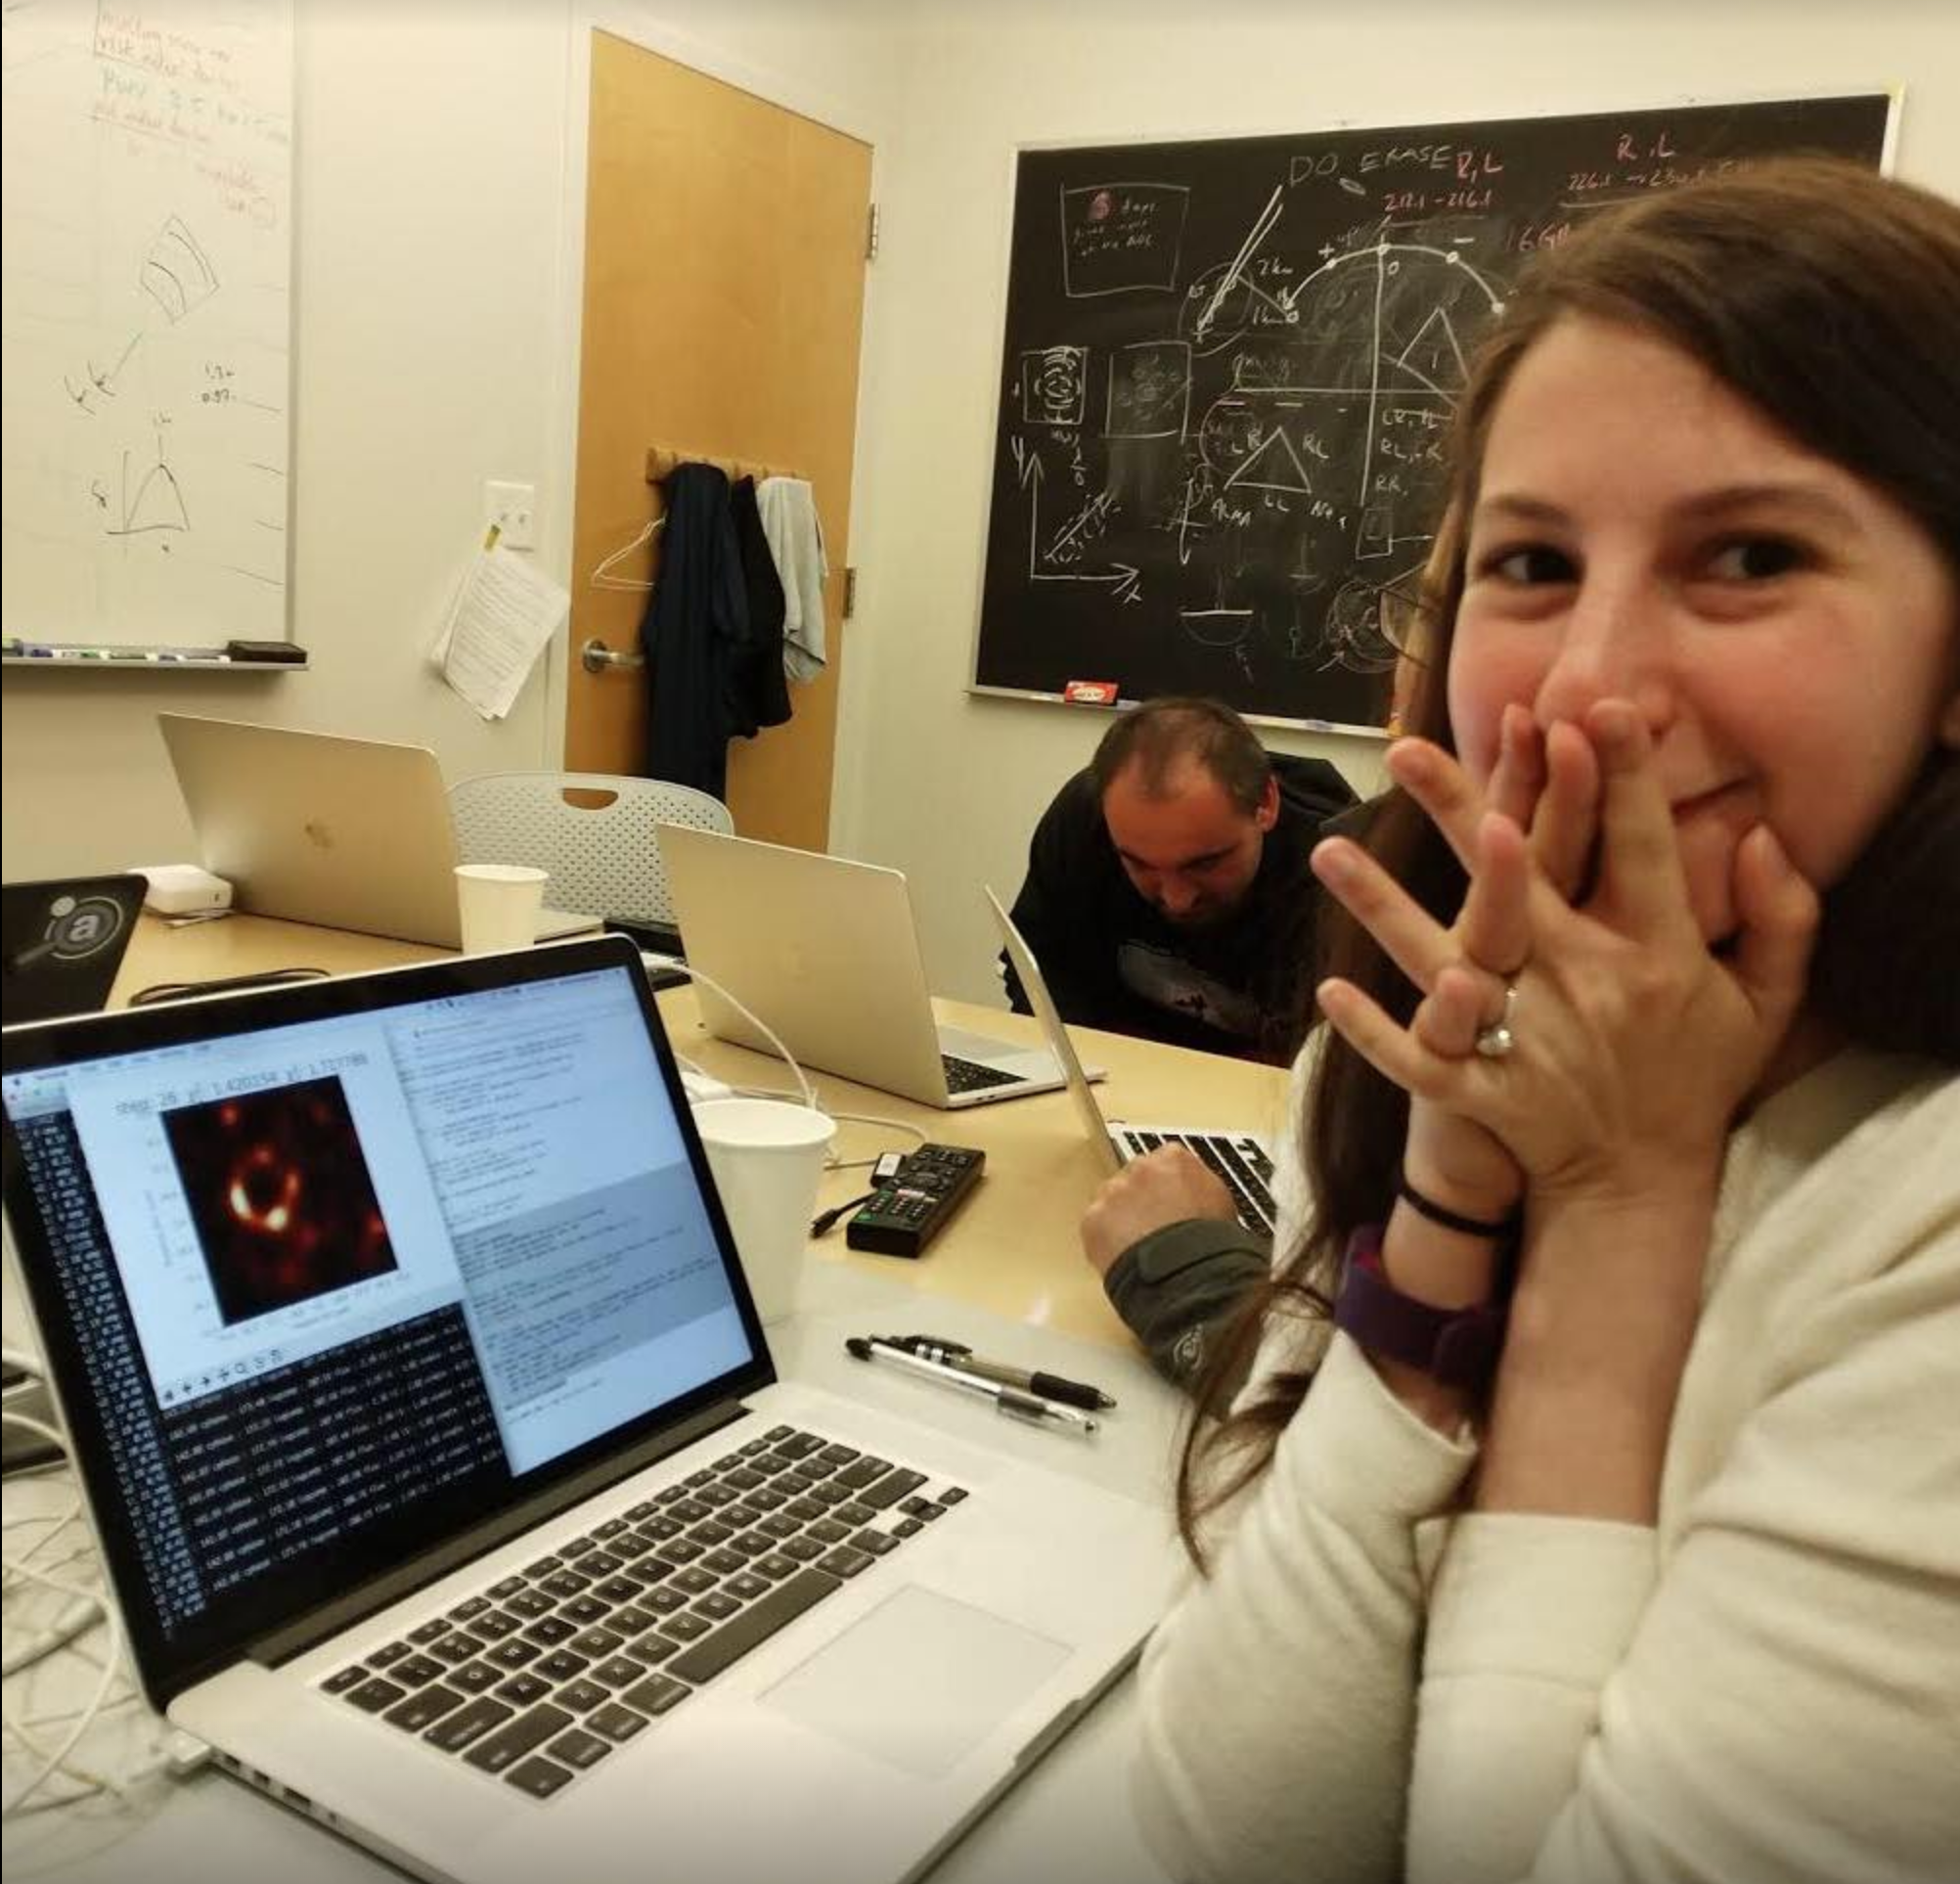
\includegraphics[width=3.98958in,height=\textheight,keepaspectratio]{index_files/mediabag/a1cd57e2943a4dd49146.png}

}

\caption{\label{fig-result-dataset}Cómo Katie Bouman se convirtió
accidentalmente en el rostro del proyecto del agujero negro.}

\end{figure}%

\section{3.2 Evidence for Multi-Reservoir
System}\label{evidence-for-multi-reservoir-system}

Our comprehensive analysis reveals three distinct seismic signatures
that strongly support the proposed multi-reservoir magma system:

\section{3.3 Pre-Eruptive Shallow Swarm
Activity}\label{pre-eruptive-shallow-swarm-activity}

Intense earthquake swarms occurred in the shallow subsurface
(\textless{} 10 km depth) during the weeks preceding the September 19th
eruption onset. This activity correlates with significant surface
deformation measurements and indicates shallow magma intrusion processes
.

\section{3.4 Syn- and Post-Eruptive Crustal Reservoir
Activity}\label{syn--and-post-eruptive-crustal-reservoir-activity}

Following eruption initiation, continuous moderate-magnitude seismicity
established at 10-15 km depth, consistent with ongoing magma movement
within the proposed shallow crustal reservoir. This persistent activity
suggests active magma storage and transport processes {[}4{]}.

\begin{Shaded}
\begin{Highlighting}[]
\CommentTok{\# Instalar plotly si no está instalado}
\ControlFlowTok{if}\NormalTok{ (}\SpecialCharTok{!}\FunctionTok{require}\NormalTok{(}\StringTok{"plotly"}\NormalTok{)) \{}
  \FunctionTok{install.packages}\NormalTok{(}\StringTok{"plotly"}\NormalTok{)}
  \FunctionTok{library}\NormalTok{(plotly)}
\NormalTok{\}}

\FunctionTok{library}\NormalTok{(plotly)}

\NormalTok{fig }\OtherTok{\textless{}{-}} \FunctionTok{plot\_ly}\NormalTok{(}
    \AttributeTok{type =} \StringTok{\textquotesingle{}scatterpolar\textquotesingle{}}\NormalTok{,}
    \AttributeTok{fill =} \StringTok{\textquotesingle{}toself\textquotesingle{}}
\NormalTok{  )}
\NormalTok{fig }\OtherTok{\textless{}{-}}\NormalTok{ fig }\SpecialCharTok{\%\textgreater{}\%}
  \FunctionTok{add\_trace}\NormalTok{(}
    \AttributeTok{r =} \FunctionTok{c}\NormalTok{(}\DecValTok{39}\NormalTok{, }\DecValTok{28}\NormalTok{, }\DecValTok{8}\NormalTok{, }\DecValTok{7}\NormalTok{, }\DecValTok{28}\NormalTok{, }\DecValTok{39}\NormalTok{),}
    \AttributeTok{theta =} \FunctionTok{c}\NormalTok{(}\StringTok{\textquotesingle{}A\textquotesingle{}}\NormalTok{,}\StringTok{\textquotesingle{}B\textquotesingle{}}\NormalTok{,}\StringTok{\textquotesingle{}C\textquotesingle{}}\NormalTok{, }\StringTok{\textquotesingle{}D\textquotesingle{}}\NormalTok{, }\StringTok{\textquotesingle{}E\textquotesingle{}}\NormalTok{, }\StringTok{\textquotesingle{}A\textquotesingle{}}\NormalTok{),}
    \AttributeTok{name =} \StringTok{\textquotesingle{}Group A\textquotesingle{}}
\NormalTok{  )}
\NormalTok{fig }\OtherTok{\textless{}{-}}\NormalTok{ fig }\SpecialCharTok{\%\textgreater{}\%}
  \FunctionTok{add\_trace}\NormalTok{(}
    \AttributeTok{r =} \FunctionTok{c}\NormalTok{(}\FloatTok{1.5}\NormalTok{, }\DecValTok{10}\NormalTok{, }\DecValTok{39}\NormalTok{, }\DecValTok{31}\NormalTok{, }\DecValTok{15}\NormalTok{, }\FloatTok{1.5}\NormalTok{),}
    \AttributeTok{theta =} \FunctionTok{c}\NormalTok{(}\StringTok{\textquotesingle{}A\textquotesingle{}}\NormalTok{,}\StringTok{\textquotesingle{}B\textquotesingle{}}\NormalTok{,}\StringTok{\textquotesingle{}C\textquotesingle{}}\NormalTok{, }\StringTok{\textquotesingle{}D\textquotesingle{}}\NormalTok{, }\StringTok{\textquotesingle{}E\textquotesingle{}}\NormalTok{, }\StringTok{\textquotesingle{}A\textquotesingle{}}\NormalTok{),}
    \AttributeTok{name =} \StringTok{\textquotesingle{}Group B\textquotesingle{}}
\NormalTok{  )}
\NormalTok{fig }\OtherTok{\textless{}{-}}\NormalTok{ fig }\SpecialCharTok{\%\textgreater{}\%}
  \FunctionTok{layout}\NormalTok{(}
    \AttributeTok{polar =} \FunctionTok{list}\NormalTok{(}
      \AttributeTok{radialaxis =} \FunctionTok{list}\NormalTok{(}
        \AttributeTok{visible =} \ConstantTok{TRUE}\NormalTok{,}
        \AttributeTok{range =} \FunctionTok{c}\NormalTok{(}\DecValTok{0}\NormalTok{,}\DecValTok{50}\NormalTok{)}
\NormalTok{      )}
\NormalTok{    )}
\NormalTok{  )}

\NormalTok{fig}
\end{Highlighting}
\end{Shaded}

\section{3.5 Deep Mantle Reservoir
Signatures}\label{deep-mantle-reservoir-signatures}

High-magnitude seismic events (M \textgreater{} 4.0) occurred
systematically at 30-40 km depths throughout the study period. These
deeper events, while less frequent than shallow activity, demonstrate
continuous activity within the proposed deep mantle reservoir system.

\begin{Shaded}
\begin{Highlighting}[]
\NormalTok{//| echo: false}
\NormalTok{//| label: fig{-}radar}
\NormalTok{//| fig{-}cap: "Gráfico radar de 30 indicadores de resiliencia comunitaria. Lorem ipsum dolor sit amet, consectetur adipiscing elit. Praesent tincidunt, arcu vitae suscipit commodo.Lorem ipsum dolor sit amet, consectetur adipiscing elit. Praesent tincidunt, arcu vitae suscipit commodo"}
\NormalTok{// Datos: 30 indicadores con su valor (aquí puse valores ficticios que puedes reemplazar)}
\NormalTok{data = [}
\NormalTok{  \{axis: "1. Evaluación comunitaria", value: 1.2\},}
\NormalTok{  \{axis: "2. Evaluación científica del riesgo", value: 2.0\},}
\NormalTok{  \{axis: "3. Diseminación de información en RRD", value: 2.5\},}
\NormalTok{  \{axis: "4. Educación de los niños en RRD", value: 3.0\},}
\NormalTok{  \{axis: "5. RRD en la planificación del desarrollo", value: 1.8\},}
\NormalTok{  \{axis: "6. RRD en la planificación territorial", value: 2.0\},}
\NormalTok{  \{axis: "7. Toma comunitaria de decisiones", value: 2.2\},}
\NormalTok{  \{axis: "8. Inclusión de grupos vulnerables", value: 1.7\},}
\NormalTok{  \{axis: "9. Participación de las mujeres", value: 2.3\},}
\NormalTok{  \{axis: "10. Conocimiento de derechos", value: 1.9\},}
\NormalTok{  \{axis: "11. Alianzas para la RRD", value: 2.6\},}
\NormalTok{  \{axis: "12. Gestión ambiental sostenible", value: 2.1\},}
\NormalTok{  \{axis: "13. Seguridad y gestión del agua", value: 1.8\},}
\NormalTok{  \{axis: "14. Acceso y conciencia de la salud", value: 1.6\},}
\NormalTok{  \{axis: "15. Suministro seguro de alimentos", value: 1.4\},}
\NormalTok{  \{axis: "16. Prácticas de medios de vida", value: 1.3\},}
\NormalTok{  \{axis: "17. Acceso a mercado", value: 1.5\},}
\NormalTok{  \{axis: "18. Acceso a servicios financieros", value: 1.2\},}
\NormalTok{  \{axis: "19. Protección de ingresos y activos", value: 1.7\},}
\NormalTok{  \{axis: "20. Acceso a protección social", value: 2.0\},}
\NormalTok{  \{axis: "21. Cohesión social", value: 3.2\},}
\NormalTok{  \{axis: "22. Infraestructura crítica", value: 2.8\},}
\NormalTok{  \{axis: "23. Vivienda", value: 1.9\},}
\NormalTok{  \{axis: "24. Planificación de contingencia", value: 2.1\},}
\NormalTok{  \{axis: "25. Sistema de alerta temprana", value: 2.3\},}
\NormalTok{  \{axis: "26. Capacidad de preparación", value: 2.0\},}
\NormalTok{  \{axis: "27. Servicios de salud", value: 2.5\},}
\NormalTok{  \{axis: "28. Servicios de educación", value: 2.9\},}
\NormalTok{  \{axis: "29. Infraestructura en emergencias", value: 2.7\},}
\NormalTok{  \{axis: "30. Liderazgo y voluntariado", value: 3.0\}}
\NormalTok{]}

\NormalTok{// Radar chart con D3}
\NormalTok{\{}
\NormalTok{  const width = 550, height = 550;}
\NormalTok{  const radius = Math.min(width, height) / 2 {-} 60;}
\NormalTok{  const levels = 5; // número de círculos concéntricos}
\NormalTok{  const maxValue = 3.5; // escala máxima}

\NormalTok{  const angleSlice = (Math.PI * 2) / data.length;}

\NormalTok{  const rScale = d3.scaleLinear()}
\NormalTok{    .domain([0, maxValue])}
\NormalTok{    .range([0, radius]);}

\NormalTok{  const svg = d3.create("svg")}
\NormalTok{    .attr("width", width)}
\NormalTok{    .attr("height", height);}

\NormalTok{  const g = svg.append("g")}
\NormalTok{    .attr("transform", \textasciigrave{}translate($\{width/2\},$\{height/2\})\textasciigrave{});}

\NormalTok{  // Dibujar círculos concéntricos}
\NormalTok{  for (let i = 0; i \textless{}= levels; i++) \{}
\NormalTok{    g.append("circle")}
\NormalTok{      .attr("r", radius/levels * i)}
\NormalTok{      .attr("fill", "none")}
\NormalTok{      .attr("stroke", "\#ccc");}
\NormalTok{  \}}

\NormalTok{  // Ejes radiales}
\NormalTok{  data.forEach((d, i) =\textgreater{} \{}
\NormalTok{    const angle = angleSlice * i {-} Math.PI/2;}
\NormalTok{    g.append("line")}
\NormalTok{      .attr("x1", 0)}
\NormalTok{      .attr("y1", 0)}
\NormalTok{      .attr("x2", rScale(maxValue) * Math.cos(angle))}
\NormalTok{      .attr("y2", rScale(maxValue) * Math.sin(angle))}
\NormalTok{      .attr("stroke", "\#999");}

\NormalTok{    // Etiquetas}
\NormalTok{    g.append("text")}
\NormalTok{      .attr("x", (rScale(maxValue + 0.2)) * Math.cos(angle))}
\NormalTok{      .attr("y", (rScale(maxValue + 0.2)) * Math.sin(angle))}
\NormalTok{      .attr("dy", "0.35em")}
\NormalTok{      .style("font{-}size", "10px")}
\NormalTok{      .style("text{-}anchor", angle \textgreater{} Math.PI/2 \&\& angle \textless{} 3*Math.PI/2 ? "end" : "start")}
\NormalTok{      .text(d.axis);}
\NormalTok{  \});}

\NormalTok{  // Línea de valores}
\NormalTok{  const line = d3.lineRadial()}
\NormalTok{    .radius(d =\textgreater{} rScale(d.value))}
\NormalTok{    .angle((d,i) =\textgreater{} i * angleSlice)}
\NormalTok{    .curve(d3.curveLinearClosed);}

\NormalTok{  g.append("path")}
\NormalTok{    .datum(data)}
\NormalTok{    .attr("d", line)}
\NormalTok{    .attr("fill", "rgba(50,150,250,0.5)")}
\NormalTok{    .attr("stroke", "steelblue")}
\NormalTok{    .attr("stroke{-}width", 2);}

\NormalTok{  return svg.node();}
\NormalTok{\}}
\end{Highlighting}
\end{Shaded}

\bookmarksetup{startatroot}

\chapter{4. DISCUSIÓN}\label{discusiuxf3n}

\section{4.1 Validation of Multi-Reservoir
Models}\label{validation-of-multi-reservoir-models}

The seismic evidence presented strongly validates theoretical
multi-reservoir magma storage models previously proposed for Cumbre
Vieja. The bimodal depth distribution of earthquakes, with distinct
clustering at shallow (10-15 km) and deep (30-40 km) levels, provides
compelling observational support for hierarchical magma storage systems
{[}5{]}.

\section{4.2 Implications for Volcanic Hazard
Assessment}\label{implications-for-volcanic-hazard-assessment}

Understanding magma reservoir architecture has direct implications for
eruption forecasting:

\begin{itemize}
\tightlist
\item
  \textbf{Deep reservoir monitoring}: High-magnitude events at mantle
  depths may serve as long-term eruption precursors
\item
  \textbf{Shallow reservoir dynamics}: Swarm activity in the crustal
  reservoir provides short-term eruption warnings
\item
  \textbf{System connectivity}: Temporal relationships between deep and
  shallow activity indicate reservoir interaction
\end{itemize}

\section{4.3 Methodological Advances}\label{methodological-advances}

This study demonstrates the effectiveness of systematic seismic catalog
analysis for validating geophysical models. The integration of spatial,
temporal, and magnitude characteristics provides a robust framework for
magma system characterization.

\bookmarksetup{startatroot}

\chapter{5. CONCLUSIONES}\label{conclusiones}

Analysis of 5,465 seismic events from the 2021 La Palma eruption
provides unprecedented insight into active volcanic processes:

\begin{tcolorbox}[enhanced jigsaw, colframe=quarto-callout-important-color-frame, rightrule=.15mm, toprule=.15mm, arc=.35mm, opacityback=0, leftrule=.75mm, breakable, left=2mm, bottomrule=.15mm, colback=white]

Puntos Clave

\begin{itemize}
\tightlist
\item
  Lorem ipsum dolor sit amet, consectetur adipiscing elit. Praesent
  tincidunt, arcu vitae suscipit commodo.
\item
  Lorem ipsum dolor sit amet, consectetur adipiscing elit. Praesent
  tincidunt, arcu vitae suscipit commodo.
\item
  Lorem ipsum dolor sit amet, consectetur adipiscing elit. Praesent
  tincidunt, arcu vitae suscipit commodo.
\end{itemize}

\end{tcolorbox}

\begin{tcolorbox}[enhanced jigsaw, colframe=quarto-callout-important-color-frame, rightrule=.15mm, toprule=.15mm, arc=.35mm, opacityback=0, leftrule=.75mm, breakable, left=2mm, bottomrule=.15mm, colback=white]

Preguntas por resolver

\begin{itemize}
\tightlist
\item
  Lorem ipsum dolor sit amet, consectetur adipiscing elit. Praesent
  tincidunt, arcu vitae suscipit commodo.
\item
  Lorem ipsum dolor sit amet, consectetur adipiscing elit. Praesent
  tincidunt, arcu vitae suscipit commodo.
\item
  Lorem ipsum dolor sit amet, consectetur adipiscing elit. Praesent
  tincidunt, arcu vitae suscipit commodo.
\end{itemize}

\end{tcolorbox}

\begin{tcolorbox}[enhanced jigsaw, colframe=quarto-callout-important-color-frame, rightrule=.15mm, toprule=.15mm, arc=.35mm, opacityback=0, leftrule=.75mm, breakable, left=2mm, bottomrule=.15mm, colback=white]

Recomendaciones para tomar decisiones

\begin{itemize}
\tightlist
\item
  Lorem ipsum dolor sit amet, consectetur adipiscing elit. Praesent
  tincidunt, arcu vitae suscipit commodo.
\item
  Lorem ipsum dolor sit amet, consectetur adipiscing elit. Praesent
  tincidunt, arcu vitae suscipit commodo.
\item
  Lorem ipsum dolor sit amet, consectetur adipiscing elit. Praesent
  tincidunt, arcu vitae suscipit commodo.
\end{itemize}

\end{tcolorbox}

\bookmarksetup{startatroot}

\chapter{AGRADECIMIENTOS}\label{agradecimientos}

Lorem ipsum dolor sit amet, consectetur adipiscing elit. Praesent
tincidunt, arcu vitae suscipit commodo. Lorem ipsum dolor sit amet,
consectetur adipiscing elit. Praesent tincidunt, arcu vitae suscipit
commodo. Lorem ipsum dolor sit amet, consectetur adipiscing elit.
Praesent tincidunt, arcu vitae suscipit commodo.

\bookmarksetup{startatroot}

\chapter{DECLARACIÓN DE AUTORIA
CREDIT}\label{declaraciuxf3n-de-autoria-credit}

Seismic data were obtained from the Instituto Geográfico Nacional (IGN)
public database. Data processing scripts, analysis notebooks, and
visualization tools have been developed to ensure reproducibility and
are available through institutional repositories. All methodological
approaches follow open science principles to facilitate community
validation and extension.

\bookmarksetup{startatroot}

\chapter{BIBLIOGRAFÍA}\label{bibliografuxeda}

\phantomsection\label{refs}
\begin{CSLReferences}{0}{1}
\bibitem[\citeproctext]{ref-connor2015}
\CSLLeftMargin{1. }%
\CSLRightInline{Connor C, Bebbington M, Marzocchi W. Probabilistic
Volcanic Hazard Assessment {[}Internet{]}. Elsevier Inc.; 2015.
Disponible en:
\url{http://dx.doi.org/10.1016/B978-0-12-385938-9.00051-1}}

\bibitem[\citeproctext]{ref-lindsay2018}
\CSLLeftMargin{2. }%
\CSLRightInline{Lindsay JM, Robertson REA.
\href{https://doi.org/10.3389/feart.2018.00042}{Integrating volcanic
hazard data in a systematic approach to develop volcanic hazard maps in
the lesser antilles}. Frontiers in Earth Science. 2018;6(April):1-17. }

\bibitem[\citeproctext]{ref-jenkins2014}
\CSLLeftMargin{3. }%
\CSLRightInline{Jenkins SF, Spence RJS, Fonseca JFBD, Solidum RU, Wilson
TM. Volcanic risk assessment: Quantifying physical vulnerability in the
built environment. Journal of Volcanology and Geothermal Research
{[}Internet{]}. 2014;276:105-20. Disponible en:
\url{http://dx.doi.org/10.1016/j.jvolgeores.2014.03.002}}

\bibitem[\citeproctext]{ref-woodford2015}
\CSLLeftMargin{4. }%
\CSLRightInline{Woodford KO. Global volcanic hazards and risk. 2015. }

\bibitem[\citeproctext]{ref-williams-jones2015}
\CSLLeftMargin{5. }%
\CSLRightInline{Williams-Jones G, Rymer H. Hazards of Volcanic Gases
{[}Internet{]}. Elsevier Inc.; 2015. Disponible en:
\url{http://dx.doi.org/10.1016/B978-0-12-385938-9.00057-2}}

\end{CSLReferences}

\bookmarksetup{startatroot}

\chapter*{References}\label{references}
\addcontentsline{toc}{chapter}{References}

\markboth{References}{References}

\phantomsection\label{refs}
\begin{CSLReferences}{0}{1}
\bibitem[\citeproctext]{ref-connor2015}
\CSLLeftMargin{1. }%
\CSLRightInline{Connor C, Bebbington M, Marzocchi W. Probabilistic
Volcanic Hazard Assessment {[}Internet{]}. Elsevier Inc.; 2015.
Disponible en:
\url{http://dx.doi.org/10.1016/B978-0-12-385938-9.00051-1}}

\bibitem[\citeproctext]{ref-lindsay2018}
\CSLLeftMargin{2. }%
\CSLRightInline{Lindsay JM, Robertson REA.
\href{https://doi.org/10.3389/feart.2018.00042}{Integrating volcanic
hazard data in a systematic approach to develop volcanic hazard maps in
the lesser antilles}. Frontiers in Earth Science. 2018;6(April):1-17. }

\bibitem[\citeproctext]{ref-jenkins2014}
\CSLLeftMargin{3. }%
\CSLRightInline{Jenkins SF, Spence RJS, Fonseca JFBD, Solidum RU, Wilson
TM. Volcanic risk assessment: Quantifying physical vulnerability in the
built environment. Journal of Volcanology and Geothermal Research
{[}Internet{]}. 2014;276:105-20. Disponible en:
\url{http://dx.doi.org/10.1016/j.jvolgeores.2014.03.002}}

\bibitem[\citeproctext]{ref-woodford2015}
\CSLLeftMargin{4. }%
\CSLRightInline{Woodford KO. Global volcanic hazards and risk. 2015. }

\bibitem[\citeproctext]{ref-williams-jones2015}
\CSLLeftMargin{5. }%
\CSLRightInline{Williams-Jones G, Rymer H. Hazards of Volcanic Gases
{[}Internet{]}. Elsevier Inc.; 2015. Disponible en:
\url{http://dx.doi.org/10.1016/B978-0-12-385938-9.00057-2}}

\end{CSLReferences}


\backmatter


\end{document}
